%-----------------------------------------------------------------
%	CONCLUSIONS
%	!TEX root = ./../main.tex
%-----------------------------------------------------------------
\section{Results and Discussion}\label{sec:res}

Results of the preceding implementation in \Cref{sec:implementation} will be presented in this section. Mainly, the objective of this analysis is finding optimal path from Barcelona to Sevilla. In \cref{fig:bcntosevilla}, it is shown the map of optimal path computed with the distance \SI{958815.01}{\m} with a number of optimal nodes of \num{6649} as seen in \cref{tab:results}. As a performance indicator, we used \inline{perf stat}; the program took around \SI{11.972}{\s} to obtain and print the optimal path to a \inline{solution.csv} file. 
\begin{figure}[H]
    \centering
    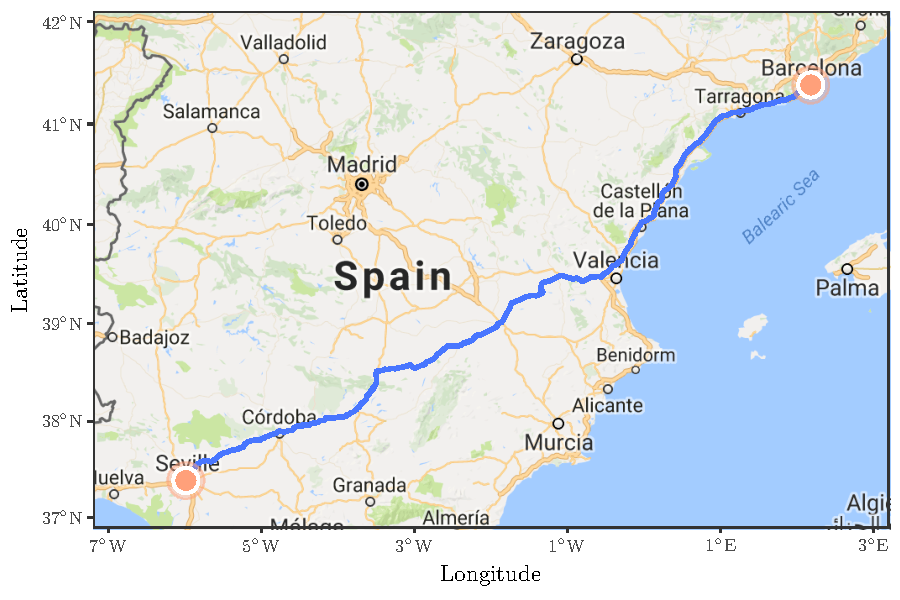
\includegraphics[width=0.9\textwidth]{images/solution}
    \caption{Optimal Path from Barcelona to Sevilla}
    \label{fig:bcntosevilla}
\end{figure}

\begin{table}[H]
  \centering
  \begin{tabular}{l c}
      \toprule
      \toprule
      Creating the binary file                  & \SI{28.817}{\s} \\
      Creating the binary file (\texttt{Ofast}) & \SI{28.732}{\s} \\
      Finding the optimal path                  & \SI{11.972}{\s} \\
      Finding the optimal path (\texttt{Ofast}) & \SI{8.599}{\s}  \\
      \midrule
      Optimal path distance    & \SI{958815.01}{\m} \\
      Number of nodes          & \num{6649} \\
      \bottomrule
  \end{tabular}
  \caption{Information about the Performance and Results of Implemented Program}
  \label{tab:results}
\end{table}

In case one wanted to apply the A* Algorithm to two arbitrary nodes in Spain, we have implemented another version of the main program (\inline{a-star-input.c}) that allows the user to select the start and goal nodes\footnote{One can easily find node IDs using \url{https://nominatim.openstreetmap.org}, or grepping the \texttt{.csv} database}. 

To test this interactive version of the program, we tried to find the optimal path in smaller area using the implemented algorithm from Barcelona (node \inline{240949599}) to UAB (node \inline{255403621}):
\begin{lstlisting}[language=bash]
gcc -lm -Ofast functions.c a-star-input.c -o astar-input
./astar-input 240949599 255403621
\end{lstlisting}

The optimal path computed is illustrated in \cref{fig:bcntouab}. The distance is around \SI{19839.10}{\m} with the number of nodes is \num{331}, and the program need about \SI{0.916}{\s} to get the results as summarized in \cref{tab:results-uab}.

\begin{figure}[H]
    \centering
    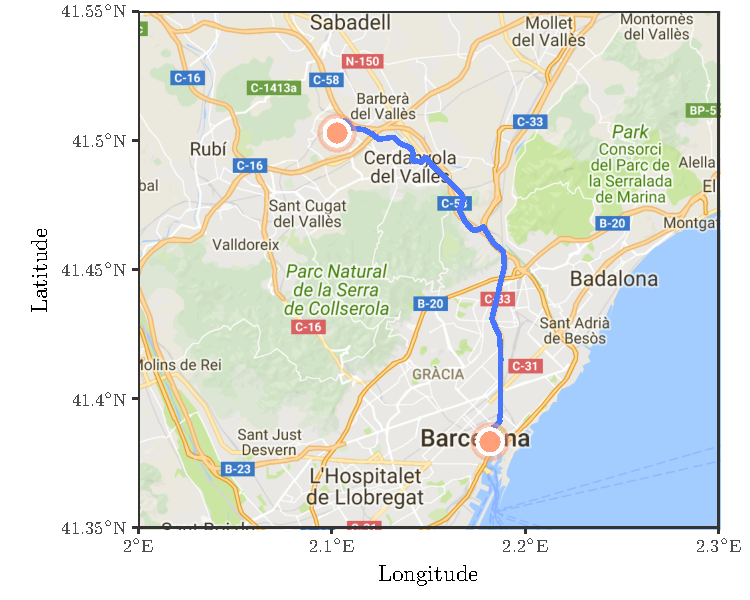
\includegraphics[width=0.8\textwidth]{images/solution-uab}
    \caption{Optimal Path from Barcelona to UAB}
    \label{fig:bcntouab}
\end{figure}


\begin{table}[H]
  \centering
  \begin{tabular}{l c}
      \toprule
      \toprule
      Finding the optimal path                  & \SI{0.916}{\s} \\
      Finding the optimal path (\texttt{Ofast}) & \SI{0.819}{\s} \\
      \midrule
      Optimal path distance    & \SI{19839.10}{\m} \\
      Number of nodes          & \num{331} \\
      \bottomrule
  \end{tabular}
  \caption{Information about the Performance and Results of Implemented Program}
  \label{tab:results-uab}
\end{table}

\newpage
\subsection{Further Improvements}

Some different experiments, for instance changing the heuristic functions have been left for the future work due to lack of time. There are some ideas that we would like to try during the implementation of A* algorithm. This analysis report mainly focused on finding path from Barcelona to Sevilla, leaving the finding optimal path from different places. For this reason, we propose some ideas to be tested and implemented as part of future work and further improvements as follows:
\begin{enumerate}[(i)]
	\item Try different heuristic functions and compare the performance of the algorithm.
    \item Include larger area to be tested to find optimal path, for instance whole area of Europe (we are not even sure the whole Spain area is included, as some of the nodes we tried to experiment with were not in the \inline{.csv} file).
    \item For the latter, we would like to define some of the variables in a less \emph{hardcoded} way, especially when dealing with sizes memory allocation.
    \item Trying to find an optimal path from Barcelona to Madrid the A* Algorithm got apparently stuck in a cyclic loop at some point. This is because a node in the \inline{CLOSED} list could end up back again in the \inline{OPEN} list. This is an issue that would be interesting to address.
	\item Improve the performance of the programs in terms of memory. Surely some variables could have been freed after not needing them anymore.
%     \item Implementing Jump Point Search (JPS) which is an optimization to the A* search algorithm for uniform-cost grids.
\end{enumerate}


